\chapter{Argomento: Somma di due dadi}
{ }\hfill\textbf{Livello:} Medio\\ \\
Lanciando due dadi, la somma dei punti sulla loro faccia superiore è un numero intero compreso tra 2 e 12. Il programma calcolerà le diverse probabilità di apparire di ciascun numero e le rappresenterà in un grafico.


\section{Simulare il lancio di un dado.}
Per simulare il lancio di un dado useremo la primitiva \texttt{Casuale}. Ecco come funziona: \\

\texttt{Casuale 6} $\longrightarrow$ restituisce un numero intero compreso tra 0 e 5 (0, 1, 2, 3, 4, 5). Quindi \texttt{(Casuale 6)+1 } restituisce un intero a caso tra 1 e 6. Le parentesi sono necessarie perché altrimenti \logo\ sommerebbe 6+1 e restituirebbe un numero casuale tra 0 e 6. Per evitare di scrivere le parentesi potremmo scrivere \texttt{1+Casuale~6}. \\
Definiamo la procedura chiamata \texttt{dado} che simula il lancio di un dado.
\begin{lstlisting}
Per dado
	Output 1+Casuale 6
Fine
\end{lstlisting}


\section{Il programma}
Useremo la modalità multitartaruga e la primitiva \texttt{ImpostaTartaruga}. \texttt{ImpostaTartaruga} seguito da un numero intero ci permette di selezionare la tartaruga identificata dal numero stesso.\\
Uno schema è meglio di mille parole\textellipsis
\begin{center}
	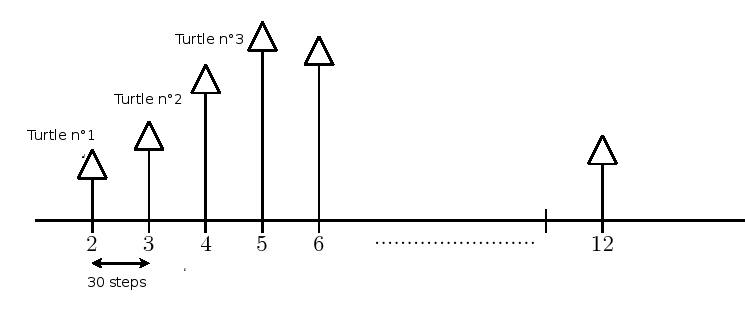
\includegraphics[scale=0.45]{pics/somme-des-schema.png}
\end{center}
\vspace{0.5cm}

Ciascuna tartaruga il cui numero va da 2 a 12 avanzerà di un passo quando la somma delle facce dei dadi appare. Per esempio, se i due dadi totalizzano 8 allora la tartaruga 8 avanzerà di un passo. Tra due tartarughe successive ci sono 30 passi orizzontalmente.\\
Impostiamo tutte le tartarughe usando le coordinate.
\begin{itemize}
	\item  La tartaruga numero 2 ha coordinate $(-150;0)$
	\item  La tartaruga numero 3 ha coordinate $(-120;0)$
	\item  La tartaruga numero 4 ha coordinate $(-90;0)$
	\item  La tartaruga numero 5 ha coordinate $(-60;0)$\\
	\begin{minipage}{8 cm}
		\begin{center}
			$\vdots$
		\end{center}
	\end{minipage}
\end{itemize}

\begin{lstlisting}
	ImpostaTartaruga 2 ImpPos [-150 0]
	ImpostaTartaruga 3 ImpPos [-120 0]
	ImpostaTartaruga 4 ImpPos [-90 0]
	ImpostaTartaruga 5 ImpPos [-60 0]
	ImpostaTartaruga 6 ImpPos [-30 0]
	...
\end{lstlisting}

Meglio di scrivere per 11 volte la stessa linea di comandi usiamo la primitiva \texttt{RipetiPer}. Con questa primitiva possiamo assegnare ad una variabile una sequenza di valori. In questo caso vogliamo assegnare alla variabile \texttt{:i} valori successivi da 2 a 12. Scriviamo:
\texttt{RipetiPer [i 2 12] [ elenco di istruzioni ]}\\

Per impostare tutte le tartarughe creiamo la procedura \texttt{inizializza}
\begin{lstlisting}
per inizializza
	PulisciSchermo NascondiTartaruga PennaSu
	RipetiPer [i 2 12] [ 
		ImpostaTartaruga :i ImpPos Elenco -150+(:i-2)*30 0
		PennaSu Indietro 15 Etichetta :i Avanti 15 PennaGiu 
	]
fine
\end{lstlisting}

Cerchiamo di capire l'espressione \texttt{-150+(:i-2)*30}. Iniziamo da $-150$ e, per ogni nuova tartaruga, aggiungiamo 30 (verificalo con diversi valori di \texttt{:i} se sei scettico).\\
Infine questo è il programma:

\begin{lstlisting}
Per dado
	output 1+Casuale 6
Fine

per inizializza
	PulisciSchermo NascondiTartaruga PennaSu
	RipetiPer [i 2 12] [ 
		ImpostaTartaruga :i ImpPos Elenco -150+(:i-2)*30 0
		PennaSu Indietro 15 Etichetta :i Avanti 15 PennaGiu 
	]
fine

per avvia
	inizializza
	Ripeti 1000 [
		AssegnaVar "sum dado+dado
		impostatartaruga :sum Avanti 1
	]
	RipetiPer [i 2 12] [
		impostatartaruga :i
		# le coordtinate y di ciascuna tartaruga 
		# rappresenta in numero di volte che il numero
		# e' apparso
		AssegnaVarLocale "number Ultimo Posizione 
		PennaSu Avanti 10 RuotaSinistra 90 Avanti 10 
		RuotaDestra 90 PennaGiu Etichetta :number/1000*100
	]
fine
\end{lstlisting}

Qui c'è un programma più generale. Chiederemo all'utente il numero di dadi e quello di lanci.
\begin{lstlisting}
per inizializza
	PulisciSchermo NascondiTartaruga PennaSu ImpNumMaxT :max+1
	RipetiPer Frase Elenco "i :min :max [ 
		ImpTar :i ImpPos Elenco -150+(:i-2)*30 0
		PennaSu Indietro 15 Etichetta :i Avanti 15 PennaGiu 
	]
fine

per dado
	AssegnaVarLocale "somma 0
	Ripeti :dice [
		AssegnaVarLocale "somma :somma+1+Casuale 6
	]
	Output :somma
fine

per avvia
	Leggi [Numero di dadi:] "dice
	Se non Numero? :dice [Stampa [Non e' un numero valido!] Ferma]
	AssegnaVar "min :dice
	AssegnaVar "max 6*:dice
	Leggi [Numero di lanci: ] "lanci
	Se non Numero? :lanci [Stampa [Non e' un numero valido] Ferma]
	inizializza
	Ripeti :lanci [
		impostatartaruga dado Avanti 1
	]
	RipetiPer Frase Elenco "i :min :max [
		impostatartaruga :i
		AssegnaVarLocale "effectif Ultimo Posizione 
		# Arrotonda per 0.1
		PennaSu Avanti 10 RuotaSinistra 90 Avanti 10 RuotaDestra 90 
		PennaGiu Etichetta (Arrotonda :effectif/:lanci*1000)/10
	]
fine
\end{lstlisting}